% Copyright (C) 2014-2020 by Thomas Auzinger <thomas@auzinger.name>

\documentclass[draft,final]{vutinfth} % Remove option 'final' to obtain debug information.

% Load packages to allow in- and output of non-ASCII characters.
\usepackage{lmodern}        % Use an extension of the original Computer Modern font to minimize the use of bitmapped letters.
\usepackage[T1]{fontenc}    % Determines font encoding of the output. Font packages have to be included before this line.
\usepackage[utf8]{inputenc} % Determines encoding of the input. All input files have to use UTF8 encoding.

% Extended LaTeX functionality is enables by including packages with \usepackage{...}.
\usepackage{amsmath}    % Extended typesetting of mathematical expression.
\usepackage{amssymb}    % Provides a multitude of mathematical symbols.
\usepackage{mathtools}  % Further extensions of mathematical typesetting.
\usepackage{microtype}  % Small-scale typographic enhancements.
\usepackage[inline]{enumitem} % User control over the layout of lists (itemize, enumerate, description).
\usepackage{multirow}   % Allows table elements to span several rows.
\usepackage{booktabs}   % Improves the typesettings of tables.
\usepackage{subcaption} % Allows the use of subfigures and enables their referencing.
\usepackage[ruled,linesnumbered,algochapter]{algorithm2e} % Enables the writing of pseudo code.
\usepackage[usenames,dvipsnames,table]{xcolor} % Allows the definition and use of colors. This package has to be included before tikz.
\usepackage{nag}       % Issues warnings when best practices in writing LaTeX documents are violated.
\usepackage{hyperref}  % Enables cross linking in the electronic document version. This package has to be included second to last.
\usepackage[acronym,toc]{glossaries} % Enables the generation of glossaries and lists fo acronyms. This package has to be included last.
\usepackage{natbib}
\usepackage{amsfonts}

% Define convenience functions to use the author name and the thesis title in the PDF document properties.
\newcommand{\authorname}{Rafael Sterzinger} % The author name without titles.
\newcommand{\thesistitle}{Balancing Extrinsic and Intrinsic Rewards in Reinforcement Learning}
%Prediction Error based Curiosity and How to Combine Extrinsic and Intrinsic Rewards
\newcommand{\thesissubtitle}{}% The title of the thesis. The English version should be used, if it exists.
\newcommand{\p}[1]{see p. #1}

% Set PDF document properties
\hypersetup{
pdfpagelayout   = TwoPageRight,           % How the document is shown in PDF viewers (optional).
linkbordercolor = {Melon},                % The color of the borders of boxes around crosslinks (optional).
pdfauthor       = {\authorname},          % The author's name in the document properties (optional).
pdftitle        = {\thesistitle},         % The document's title in the document properties (optional).
pdfsubject      = {Subject},              % The document's subject in the document properties (optional).
pdfkeywords     = {a, list, of, keywords} % The document's keywords in the document properties (optional).
}

\setpnumwidth{2.5em}        % Avoid overfull hboxes in the table of contents (see memoir manual).
\setsecnumdepth{subsection} % Enumerate subsections.

\nonzeroparskip             % Create space between paragraphs (optional).
\setlength{\parindent}{0pt} % Remove paragraph identation (optional).

\makeindex      % Use an optional index.
\makeglossaries % Use an optional glossary.
%\glstocfalse   % Remove the glossaries from the table of contents.

% Set persons with 4 arguments:
%  {title before name}{name}{title after name}{gender}
%  where both titles are optional (i.e. can be given as empty brackets {}).
\setauthor{}{\authorname}{}{male}
\setauthorextra
\setadvisor{Ao.Univ.Prof. Dipl.-Ing. Dr.techn.}{Thomas Grechenig}{}{male}

% For bachelor and master theses:
\setfirstassistant{Dipl.-Ing.}{Michael Ressmann}{Posttitle}{male}

% For dissertations:
%\setfirstreviewer{Pretitle}{Forename Surname}{Posttitle}{male}
%\setsecondreviewer{Pretitle}{Forename Surname}{Posttitle}{male}

% For dissertations at the PhD School and optionally for dissertations:
%\setsecondadvisor{Pretitle}{Forename Surname}{Posttitle}{male} % Comment to remove.

% Required data.
\setregnumber{11778282}
\setdate{10}{08}{2020} % Set date with 3 arguments: {day}{month}{year}.
\settitle{\thesistitle}{\thesistitle} % Sets English and German version of the title (both can be English or German). If your title contains commas, enclose it with additional curvy brackets (i.e., {{your title}}) or define it as a macro as done with \thesistitle.
\setsubtitle{\thesissubtitle}{\thesissubtitle} % Sets English and German version of the subtitle (both can be English or German).

% Select the thesis type: bachelor / master / doctor / phd-school.
% Bachelor:
\setthesis{bachelor}
%
% Master:
%\setthesis{master}
%\setmasterdegree{dipl.} % dipl. / rer.nat. / rer.soc.oec. / master
%
% Doctor:
%\setthesis{doctor}
%\setdoctordegree{rer.soc.oec.}% rer.nat. / techn. / rer.soc.oec.
%
% Doctor at the PhD School
%\setthesis{phd-school} % Deactivate non-English title pages (see below)

% For bachelor and master:
\setcurriculum{Business Informatics }{Wirtschaftsinformatik} % Sets the English and German name of the curriculum.

% For dissertations at the PhD School:
%\setfirstreviewerdata{Affiliation, Country}
%\setsecondreviewerdata{Affiliation, Country}


\newacronym{im}{IM}{Intrinsic Motivation}
\newacronym{em}{EM}{Extrinsic Motivation}
\newacronym{rl}{RL}{Reinforcement Learning}
\newacronym{mdp}{MDP}{Markov Decision Process}
\newacronym{ml}{ML}{Machine Learning}
\newacronym{dp}{DP}{Dynamic Programming}
\newacronym{dl}{DL}{Deep Learning}
\newacronym{drl}{DRL}{Deep Reinforcement Learning}
\newacronym{mc}{MC}{Monte-Carlo}
\newacronym{td}{TD}{Temporal-Difference}



\begin{document}

    \frontmatter % Switches to roman numbering.
%  The structure of the thesis has to conform to the guidelines at
%  https://informatics.tuwien.ac.at/study-services

    \addtitlepage{naustrian} % German title page (not for dissertations at the PhD School).
    \addtitlepage{english} % English title page.
    \addinsotitlepage{naustrian}
    \addstatementpage

    \begin{danksagung*}
    \end{danksagung*}

    \begin{acknowledgements*}
    \end{acknowledgements*}

    \begin{kurzfassung}
    \end{kurzfassung}

    \begin{abstract}
    \end{abstract}

% Select the language of the thesis, e.g., english or naustrian.
    \selectlanguage{english}

% Add a table of contents (toc).
    \tableofcontents % Starred version, i.e., \tableofcontents*, removes the self-entry.

% Switch to arabic numbering and start the enumeration of chapters in the table of content.
    \mainmatter


    \chapter{Introduction}


    \section{Problem Description}\label{sec:problem-description}
    In \gls{rl}, algorithms mainly depend on carefully designed extrinsic reward functions which are comparable with feedback to an agent's behaviour.
    In order to teach an agent a certain desired behaviour, it has to optimize this reward function by trial-and-error.
    This traditional approach yielded multiple astonishing results over the last decade.
    Task which award rewards densely, i.e.\ almost after every performed action, are common for these results.
    In opposite to dense rewards, sparse rewards are scattered in the environment which poses the problem that they occur too rarely in order for an agent to pick up the needed skills.
    An example for environments with sparse rewards are tasks which depend heavily on exploration, e.g. \textit{Montezumas's revenge}.
    \\\\
    An approach to tackle these problems is curiosity, an organism's \gls{im} to spontaneously explore its environment.
    \gls{im} allows an agent to incrementally learn valuable skills independently of its given task by an intrinsic and therefore a more general reward function.
    In general, the concept of intrinsic and extrinsic evolves around the question on why an agent performed a certain action in a given state.
    Since \gls{im} became an important part of \gls{rl}, the following challenges were crystallized out by~\cite[\p{6}]{aubret_survey_2019}:

    \begin{itemize}
        \item \textbf{Sparse rewards:} The agent never reaches a reward signal in case of sparse rewards.
        \item \textbf{State representation:} The agent does not manage to learn a representation of its observations with independent features or meaningful distance metrics.
        \item \textbf{Building option:} The agent is unable to learn abstract high-level decisions independently from the task.
        \item \textbf{Learning a curriculum:} The agent hardly defines a curriculum among its available goals without expert knowledge.
    \end{itemize}

    Besides a general introduction to \gls{im} and its challenges in \gls{rl}, this Bachelor's thesis has its focus on knowledge acquisition through exploration.
    Knowledge acquisition is described as the agents motivation to find new knowledge about its environment, meaning that it is interested in things it can or cannot control, the function of the world, discovering new areas, or understanding the proximity.
    Concerning exploration, one approach is error prediction which is the agents difficulty to predict the state following a state-action-tuple.
    This idea is heavily explored by~\cite{burda_large-scale_2018-1} and its prior work of~\cite{pathak_curiosity-driven_2017-1}, both of which are core references of this thesis.
    \\\\
    Building upon the findings of~\citeauthor{burda_large-scale_2018-1}, this Bachelor's thesis eyes on answering the question on how to optimally combine intrinsic and extrinsic rewards in order to maximize an agents score, primarily in sparse but also in dense environments.
    Furthermore, it will evaluate if a balanced reward combination tackles the noisy-TV problem, proposed by~\cite{schmidhuber_formal_2010-1}.
    The noisy-TV problem, also known as the white-noise problem, is an algorithms inability to handle the local stochasticity of the environment: "\ldots random noise in a 3D environment attracts the agent; it will passively watch the noise since it will not be able to predict the next state."\cite[\p{10}]{aubret_survey_2019}
    \\\\
    The domain of the given problem description is \gls{rl} in \gls{rl} with a focus on the model of knowledge acquisition via exploration.


    \section{Expected Results}\label{sec:expected-results}
    As aforementioned, the goal pursued by this Bachelor's thesis is to build upon the results of~\citeauthor{burda_large-scale_2018-1} and to pursue their posed question on how to optimally combine intrinsic ($r_{int}$) and extrinsic ($r_{ext}$) rewards.
    In order to do so, coefficients $\alpha$ and $\beta$ have to be selected accordingly.
    \[r=\alpha r_{int} + \beta r_{ext}\]
    From that, an optimal solution to this equation maximizes the agent's overall reward when testing.
    After a re-implementation of the proposed algorithms, the benchmarks are expected to at least match the mean rewards mentioned in the \textit{Additional Results} section from the underlying paper.
    In this section, the authors explored the performance of combined rewards on five different Atari games and already showed that the combination of rewards yield a higher mean reward.
    Therefore, an exhaustive hyper-parameter tuning should certainly improve these results.
    \\\\
    However, this raises the question on how the algorithm performs in comparison to comparable approaches such as the paper authored by~\cite{kim_emi_2019}.
    In some of the previously mentioned hard games, e.g. \textit{Frostbite}, the authors achieved only a slightly higher mean score which might be beatable by combining rewards.
    Optionally, it would be interesting to observe the performance in environments with dense rewards too since there might be an improvement to see as well.
    \\\\
    In the \textit{Discussion} section,~\citeauthor{burda_large-scale_2018-1} mention the limitations of prediction error based curiosity which was earlier introduced with the so called noisy-TV problem.
    Given this problem, the question is raised on whether or not it is possible to tackle the agent's distraction through curiosity with \gls{em}.
    This question will be pursued during the evaluation process with the posed hypothesized that it is possible to overcome an agent's distraction and the assumption that \gls{em} has a higher impact on the distraction in a densely rewarding environment than in a sparse one.
    \\\\
    With the given prospect to beat state of the art approaches to environments with sparse rewards and evaluate the amount of extrinsic reward needed to put a distracted agent back on track, it is the opportunity to pursue important constructs, which reflect the natural human propensity to learn and assimilate, in the domain of computer science that motivated this Bachelor's thesis.


    \section{Methodological Approach}\label{sec:methodological-approach}
    In order to answer the question on how to optimally combine intrinsic and extrinsic rewards, the thesis builds upon the released source code and environments from~\cite{burda_large-scale_2018-1} and~\cite{pathak_curiosity-driven_2017-1} which can be observed on these websites. \footnote{\url{https://pathak22.github.io/large-scale-curiosity}}\footnote{\url{https://pathak22.github.io/noreward-rl/}}
    Therefore, this Bachelor's thesis follows a programming approach which relies on the same tools used by the preceding authors, since it guarantees optimal reproducibility of their results.
    In an overview, these tools are the \textit{Python}\footnote{\url{https://www.python.org/}} programming language, the \gls{ml} platform \textit{TensorFlow}\footnote{\url{https://www.tensorflow.org/}}, and lastly the \textit{OpenAI Gym}\footnote{\url{https://gym.openai.com/}} which is a toolkit for developing and comparing \gls{rl} algorithms.
    \\\\
    The development progress is structured into the following five mile stones:

    \begin{enumerate}
        \item Setting-up of the environment, including the installation of the \textit{CUDA}\footnote{\url{https://developer.nvidia.com/cuda-toolkit}} toolkit and the \textit{cuDNN}\footnote{\url{https://developer.nvidia.com/cudnn}]} library
        \item Implementing a Proximal Policy Optimization (PPO) algorithm according to~\cite{schulman_proximal_2017}, using extrinsic rewards
        \item Adding an Intrinsic Curiosity Module, published by~\cite{pathak_curiosity-driven_2017-1}, in order to allow for intrinsic rewards
        \item Tuning of the coefficients $\alpha,\beta$ and comparison to state of the art approaches
        \item Recreation of the synthetic generated noisy-TV problem, proposed by~\cite{burda_large-scale_2018-1}
    \end{enumerate}

    During this incremental process, an emphasise is laid on two out of five sparse Atari games, categorized by~\cite{bellemare_unifying_2016} and picked by~\citeauthor{burda_large-scale_2018-1}.
    The initial two games are \textit{Montezumas's revenge} and \textit{Freeway}, but with the option to add the remaining ones or games with dense rewards in the future.
    \\\\
    % Eventually add VAE
    Regarding mile stone three, \textit{Random Features} and \textit{Inverse Dynamics Features} as introduced by~\citeauthor{burda_large-scale_2018-1} are primarily the focus.
    Concerning mile stone four and the comparison to state of the art approaches, the~\nameref{sec:state-of-the-art} section of this thesis allows for a current in-depth overview.
    Additionally to the aforementioned practical part, the theoretical aspect of this Bachelor's thesis will be covered by an exhaustive literature research with an emphasize on directly comparable approaches, i.e. prediction error based curiosity~\citep{burda_large-scale_2018-1}.


    \section{State of the Art}\label{sec:state-of-the-art}


    \section{Thesis Outline}\label{sec:thesis-outline}


    \chapter{Reinforcement Learning Background}\label{ch:reinforcement-learning-background}


    \section{Reinforcement Learning Problem}\label{sec:reinforcement-learning-problem}
    Reinforcement Learning, the science of decision making, is about learning the consequences of performed actions and using this knowledge to maximize a numeric \textit{reward signal} which should direct the search for a given objective~\citep{sutton_reinforcement_2018}.
    \gls{rl} problems are tackled by a learner or rather an \textit{agent} that performs actions in an \textit{environment} in a trial and error paradigm.
    The agent has no prior knowledge of the consequences of the possible actions but has to explore which action to take in a certain situation to maximize the amount of obtainable rewards.
    An additional difficulty is added if the reward for an action is delayed because the agent has to understand which of the executed actions actually led to the desirable reward it received far ahead in the future.
    Lastly, a proper weighting between exploration and exploitation has to be developed as the agent must exploit actions with known consequences to perform well but also explore new ones in order to improve~\citep{kaelbling_reinforcement_1996}.

    In addition to the aforementioned environment, agent, and reward signal, \gls{rl} consists of further subelements since it would be desirable e.g. not only to know the immediate reward but also to gain a measurement for all possible future rewards from a given state onward.
    For this purpose, a \textit{value function} is used.
    It acts as a long-term indicator that describes the attractiveness of a state an agent might result in after interacting with its environment.
    This measurement is interesting because there could be an action which leads to a high immediate reward but results in an undesirable state with no future rewards.
    Furthermore, the agent should pick up a \textit{policy} that consists of state-action tuples which should be refined and adjusted depending on the received rewards.
    Lastly, the agent may want to build a \textit{model} which estimates the environment's behaviour, in order to plan its actions in advance.
    This final addition divides the \gls{rl} problem spectrum into two parts: model-free and model-based approaches~\citep{sutton_reinforcement_2018}.


    In opposite to other known \gls{ml} disciplines such as \textit{supervised learning}, there is no supervisor in \gls{rl} that explicitly tells the agent which action would be correct in a given state and because of that, the agent has to come up with its own policy based on the repeated feedback it receives from the immediate reward and the following state~\citep{kaelbling_reinforcement_1996}.
    This spares the necessity of creating a training dataset with corresponding state-action tuples beforehand and thus \gls{rl} is the preferred choice in cases where an agent interacts with and influences its environment.
    Furthermore, teaching based on supervision would also mean that an agent will be limited to the labelling ability of the supervisor which is another reason why it must be able to learn from its own experiences~\citep{silver_lecture_2015-2}.
    Since \gls{rl} is quite distinct from supervised learning and does not rely on labelled examples, it is sometimes misclassified as \textit{unsupervised learning} which has the purpose to find structure in unlabelled data.
    However, this is not applicable for \gls{rl} as the agent has to maximize a reward function and not to find structure in data.
    Therefore, \citeauthor{sutton_reinforcement_2018} classified \gls{rl}  as a third subfield of \gls{ml}.


    \section{Markov Decision Processes}
    In order to formalize the \gls{rl} problem, the idea and notation of a \gls{mdp} is used to notate the sequential interactions between an agent and its environment.
    At every discrete time step, $t = 0,1,2,3, \ldots \in \mathbb{N}$, the agent observes the current state, $S_t \in \mathit{S}$, of the environment and selects an available action, $A_t \in \mathit{A}(s)$~\eqref{fig:rl_problem}.
    %Add note concerning R_t wich is nowadays used in DRL
    Once the agent has selected an action, it obtains a scalar reward $R_{t+1} \in \mathit{R} \subset \mathbb{R}$ and depending on the action the environment transforms into a subsequent state $S_{t+1}$.
    By means of continuous interactions between the agent and the environment a trajectory of the form $S_0,A_0,R_1,S_1,A_1,R_2,S_2,A_2,R_3,\ldots$ is created.

    \begin{figure}[h]
        \centering
        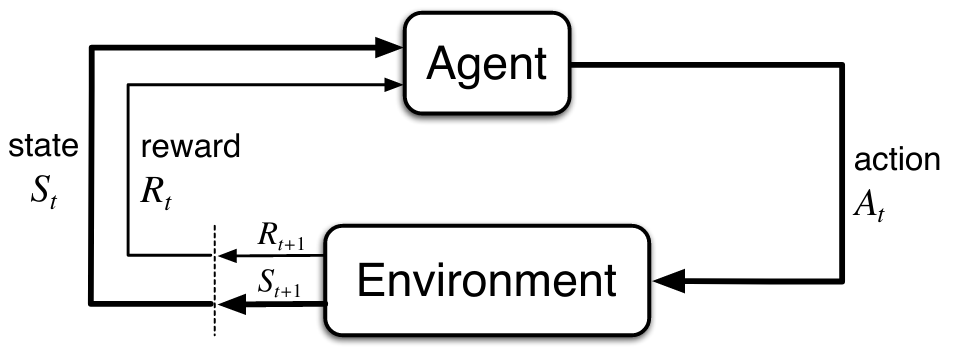
\includegraphics[width=\textwidth]{figures/rl_problem.png}
        \caption{The \gls{rl} framework formalized as a \gls{mdp}~\citep[\p{48}]{sutton_reinforcement_2018}}
        \label{fig:rl_problem}
    \end{figure}

    In a finite-horizon, the agent has to plan only a fixed number of time-steps ahead and the sets $\mathit{S},\mathit{A}\text{, and }\mathit{R}$ are limited~\citep{kaelbling_reinforcement_1996,sutton_reinforcement_2018}.
    Furthermore, the possibility that the values $s'\in \mathit{S}$ and $r \in \mathit{R}$ may occur at a time step $t+1$, can be described with a probability~\eqref{eq:distribution} solely depending on the action $a \in \mathit{A}(s)$ taken in a preceding state $s \in \mathit{S}$.

    \begin{equation}
        p(s',r|s,a) = P\{S_{t+1}=s', R_{t+1}=r | S_t=s, A_t=a\}\label{eq:distribution}
    \end{equation}

    Since $p$ describes a probability, the sum over all possible combinations of $s$ and $a$ must be equal to 1.
    Moreover, the individual probabilities of $p$ describe the dynamics of a \gls{mdp}.
    Observing this notation shows that the state $s$ must contain all the necessary information and must not depend on states preceding $s$.
    If this is the case, the state is called to have the Markov property~\eqref{eq:markov_property}~\citep{francois-lavet_introduction_2018}.

    \begin{equation}
        P\{S_{t+1}|S_t,A_t\} = P\{S_{t+1}|S_1,A_1,\ldots,S_t,A_t\} \label{eq:markov_property}
    \end{equation}

    With the notation of $p$, properties of the \gls{mdp} like the state-transition probabilities~\eqref{eq:transition} or the expected value of rewards~\eqref{eq:expected_reward} with given state-action tuples can be computed.

    \begin{equation}
        p(s'|s,a) = P\{S_{t+1}=s'| S_t=s, A_t=a\} = \sum_{r \in \mathit{R}} p(s',r | s,a) \label{eq:transition}
    \end{equation}

    \begin{equation}
        r(s',s,a) = \mathbb{E}[R_{t+1} | S_t=s, A_t=a] = \sum_{r\in \mathit{R}} r \sum_{s' \in \mathit{S}} p(s',r | s,a) \label{eq:expected_reward}
    \end{equation}

    As mentioned in the~\nameref{sec:reinforcement-learning-problem}, rewards at each time-step $R_t$ are used to formalize a goal which the agent should pursue.
    This is possible due to the reward hypothesis which states that every goal one can possibly think of, can be formalized by means of a numeric reward signal and be achieved by maximizing the cumulative long-term rewards~\citep{sutton_reinforcement_2018}.

    Mathematically, the overall reward is denoted as the sum over all rewards~\eqref{eq:sum_of_rewards}, with $T$ as the final step.

    \begin{equation}
        G_t=R_{t+1} + R_{t+2}+ \ldots + R_{T}  =\sum_{t=1}^{T} R_{t}\label{eq:sum_of_rewards}
    \end{equation}

    However, this notation is only applicable if an environment has an identifiable terminal state.
    When this state is reached, it breaks for instance a game sequence into multiple ones, where each one is called an episode.
    No matter how the agent reached the final state, the environment will reset and start over with an default initial state.

    Sometimes, this separation of episodes might not be as clear and the limit of the sequence is infinite.
    This is called a continuing task, in contrast to episodic tasks where $T$ is finite.
    Therefore, if the agent acts in an environment with a continuing task, optimizing the equation~\eqref{eq:sum_of_rewards} might not be finite.
    This issue is solved by introducing a discounting rate $\gamma$, $0 \leq \gamma \leq 1$~\citep{sutton_reinforcement_2018} which avoids infinite rewards.
    Given this discounting rate, the agent now tries to maximize the discounted sum of cumulative long-term rewards~\eqref{eq:discounted_reward}.

    \begin{equation}
        G_t = R_{t+1} + \gamma R_{t+2}+ \gamma^2 R_{t+3} + \ldots = R_{t+1} + \gamma G_{t+1} = \sum_{k=1}^{\infty} \gamma^k R_{t+k}\label{eq:discounted_reward}
    \end{equation}

    With $\gamma$ as newly introduced hyperparameter, the weighting of the rewards can be adjusted according to the given task.
    A low $\gamma$ means that the agent values more the immediate reward and rewards in the near future.
    Whereas, a high $\gamma$ forces the agent to consider long-term future rewards as well and thus the agent is more far-sighted.


    \section{Functions to Improve the Policy}\label{sec:functions-to-improve-the-policy}
    As mentioned in the~\nameref{sec:reinforcement-learning-problem} section, the policy forms an important component of the \gls{rl} framework and is usually denoted as $\pi$.
    By following a policy, the agent's probability to select a specific action at time-step $t$ is $\pi(a|s) = P\{A_t=a|S_t=s\}$ and therefore $\pi$ describes a probability distribution over actions given states~\citep{silver_lecture_2015-1}.
    Additionally, the aforementioned value function component is dependent on the policy, since $\pi$ defines which action-state tuples are considered from the current state onwards.
    Formally, the state-value function for an \gls{mdp} is denoted by $v_\pi(s)$ which stands for the expected future rewards when following the policy, starting in state $s$~\citep{sutton_reinforcement_2018}.

    \begin{equation}
        v_\pi(s) = \mathbb{E}_\pi[G_t|S_t = s] = \mathbb{E}_\pi \Bigg[\sum_{k=1}^{\infty} \gamma^k R_{t+k} \bigg| S_t = s \Bigg]\label{eq:value_function}
    \end{equation}

    In a similar way, the action-value function $q_\pi(s,a)$ of a \gls{mdp} can be defined.
    This calculates the expected future reward when the agent takes action $a$ in state $s$ and then follows the policy $\pi$.

    \begin{equation}
        q_\pi(s,a) = \mathbb{E}_\pi[G_t|S_t = s, A_t = a] = \mathbb{E}_\pi \Bigg[\sum_{k=1}^{\infty} \gamma^k R_{t+k} \bigg| S_t = s | A_t = a \Bigg]\label{eq:quality_function}
    \end{equation}

    The policy is improved by adjusting the value functions $v_\pi$ and $q_\pi$ through the agent's obtained experience.
    Since \gls{rl} aims to solve a given objective by maximizing rewards, it implicitly goes along with optimizing the agent's policy.
    If a policy $\pi$ achieves a higher value than a different policy $\pi'$, which also implies that $v_\pi(s) \geq v_{\pi'}(s), \forall s \in \mathit{S}$, then the two policies can be ordered partially, with $\pi \geq \pi'$.
    However, there can be multiple policies performing equally well~\citep{sutton_reinforcement_2018} and for any \gls{mdp} the following theorem holds true~\citep[\p{43}]{silver_lecture_2015-1}:

    \begin{itemize}
        \item There exists an optimal policy $\pi_*$ that is better than or equal to all other policies, $\pi_* \geq \pi, \forall\pi$
        \item All optimal policies achieve the optimal [state-]value function, $v_{\pi_*}(s) = v_*(s)$
        \item All optimal policies achieve the optimal action-value function, $q_{\pi_*}(s,a) = q_*(s,a)$
    \end{itemize}

    A very simple optimal policy for a given state can be derived through the action-value function $q_*(s,a)$, simply by selecting the action with the maximum value.

    \begin{equation}
        \pi_*(a|s) =
        \begin{cases}
            1 \text{ if } a =  \underset{a \in \mathit{A}}{\text{argmax}}\ q_*(s,a),\\
            0 \text{ otherwise }
        \end{cases}
    \end{equation}

    The optimal value functions are given by the following equations:

    \begin{equation}
        \begin{aligned}[t]
            v_*(s) &= \underset{\pi}{\text{max }}v_\pi(s), \forall s \in \mathit{S}, \\
            q_*(s,a) &= \underset{\pi}{\text{max }}q_\pi(s,a), \forall s \in \mathit{S} \land \forall a \in \mathit{A}\label{eq:optimal}
        \end{aligned}
    \end{equation}


    \section{Dynamic Programming}

    The value function, introduced in the previous section~\nameref{sec:functions-to-improve-the-policy}, has a similar recursive property as the equation for the discounted expected reward~\eqref{eq:discounted_reward}.
    Therefore, the value function can be expressed in an equal manner by decomposing it into the discounted descendant states $\gamma v_\pi(s')$ and the immediate reward $r$:

    \begin{equation}
        \begin{aligned}[t]
            v_\pi(s) &= \mathbb{E}_\pi[G_t|S_t=s] = \mathbb{E}_\pi[R_{t+1} + \gamma G_{t+1}|S_t=s] \\
            &  =  \sum_{a} \pi(a|s) \sum_{s'}\sum_{r} p(s',r|s,a) \bigg[r + \gamma \mathbb{E}_\pi[G_{t+1}|S_{t+1} = s'] \bigg] \\
            &  =  \sum_{a} \pi(a|s) \sum_{s'}\sum_{r} p(s',r|s,a) \bigg[r + \gamma v_{\pi}(s') \bigg], \forall s \in \mathit{S} \\
            &  =  \mathbb{E}_\pi[R_{t+1} + \gamma v_\pi(S_{t+1})|S_t=s]
            \label{eq:bellman_equation}
        \end{aligned}
    \end{equation}

    The above mentioned equation~\eqref{eq:bellman_equation} is known as the Bellman equation for $v_\pi$~\citep{sutton_reinforcement_2018} which can be directly solved due to its linearity.
    However, this calculation is only feasible for small \gls{mdp}s since its complexity is $O(n^3)$ for $n$ states~\citep{silver_lecture_2015-1}.

    For larger \gls{mdp}s exist multiple iterative solutions as for example:
    \begin{itemize}
        \item \gls{dp}
        \item \gls{mc} Evaluation
        \item \gls{td} Learning
    \end{itemize}

    The general idea of \gls{dp}, which was developed by \citeauthor{bellman_theory_1954}, is to make use of the property of recursion to simplify the complexity of calculations by storing interim results.
    In that sense, it is a method that aims at solving complex problems by breaking them down into manageable subproblems.

    All of the three above mentioned approaches are mainly used for two aspects in \gls{rl}: predicting the value function $v_\pi$ (planning) and calculating the optimal value function $v_{\pi_*}$ (controlling).
    As for \gls{dp}, an iterative process is is used.
    This process is an interplay between the Bellman equation~\eqref{eq:bellman_equation}, used to calculate the value function for a given policy, and the equations mentioned in~\eqref{eq:optimal} which update the policy~\citep{silver_lecture_2015,sutton_reinforcement_2018}.


    \section{Temporal-Difference Methods}

    %Write introduction for td using page 119 of sutton

    \subsection{Temporal Difference Prediction}
    Besides \gls{dp} and \gls{mc} evaluation, \gls{td} prediction is among one of the three mentioned techniques, combining the advantages of the other two for value function predictions.
    Firstly, it uses the benefit of bootstrapping offered by \gls{dp}~\citep{szepesvari_algorithms_2010}.
    That is the usage of predictions of the value function as the target during the learning process.
    Secondly, \gls{td} prediction directly learns from raw experience in a similar way to \gls{mc} evaluation and thus it is model-free.
    However, it only awaits the reward of one time step to form a target for the value function instead of the every-visit \gls{mc} method which awaits the fully known return for the target.

    \begin{equation}
        \begin{aligned}[t]
            \text{\gls{mc} method: } & V(S_t) \leftarrow V(S_t) + \alpha [G_t - V(S_t)]\\
            \text{\gls{td} method: } & V(S_t) \leftarrow V(S_t) + \alpha [R_{t+1} + \gamma V(S_{t+1})-V(S_t)]\\
        \end{aligned}\label{eq:td_versus_mc}
    \end{equation}

    The parameter $\alpha$ is constant which defines the step-size of each adjustment to the value function.
    The two equations express the above mentioned differences certainly well:

    \begin{quote}
        Whereas Monte Carlo methods must wait until the end of the episode to determine the increment to $V(S_t)$ (only then is $G_t$ known), TD methods need to wait only until the next time step.
        At time $t + 1$ they immediately form a target and make a useful update using the observed reward $R_{t+1}$ and the estimate $V(S_{t+1})$.

        \hfill~\cite[\p{120}]{sutton_reinforcement_2018}
    \end{quote}

    The \gls{td} method is also known as $\text{TD}(0)$ that refers to the general case $\text{TD}(\lambda)$, a method that unifies \gls{td} and \gls{mc}.

    \subsection{SARSA (On-Policy)}\label{subsec:sarsanullon-policynull}

    SARSA builds upon the idea of \gls{td} but aims to find an optimal value function and thus solve the control problem.
    In a similar manner to \gls{td}, SARSA aims to estimate the action-value function $q_\pi(s,a)$, given a current policy $\pi$.
    Since it only focuses on one policy at a time, it is also known as an on-policy algorithm.
    The action-value function is optimized by means of the following calculation:

    \begin{equation}
        Q(S_t,A_t) \leftarrow Q(S_t,A_t) + \alpha [R_{t+1} + \gamma Q(S_{t+1},A_{t+1}) - Q(S_{t},A_{t}) ]
    \end{equation}

    At each transition between the state-action tuple, the values $S_{t},A_{t},R_{t+1},S_{t+1},A_{t+1}$ are included in the optimization process, eponymous for SARSA~\citep{sutton_reinforcement_2018}.
    Under the assumption that every state-action tuple is visited infinite times and that new policies are created greedily with respect to the current action-value function, SARSA is guaranteed to converge to the optimal action-value value function and thus to the optimal policy.


    %TODO Additionally add pseudo code of sarsa

    \subsection{Q-Learning (Off-Policy)}\label{subsec:q-learningnulloff-policynull}

    Another control algorithm which is build upon the idea of \gls{td} is Q-learning which aims to directly estimate the optimal action-value function $q_*$.
    As denoted by \citeauthor{watkins_q-learning_1992}, the following calculation is used to update the action-value function $Q$.

    \begin{equation}
        Q(S_t,A_t) \leftarrow Q(S_t,A_t) + \alpha [R_{t+1} + \gamma \underset{a}{\text{max}} Q(S_{t+1},a) - Q(S_{t},A_{t}) ]
    \end{equation}

    As it does not optimize for the current policy but directly for the optimal one, Q-learning is considered an off-policy method and the policies must no be interchanged~\citep{szepesvari_algorithms_2010}.

    %TODO Additionally add pseudo code of q


    \section{Policy Gradient Methods}


    \chapter{Deep Reinforcement Learning}\label{ch:deep-reinforcement-learning}

    In the preceding chapter about the~\nameref{ch:reinforcement-learning-background}, multiple solutions to the \gls{rl} problem were presented.
    However, approaches as SARSA~\eqref{subsec:sarsanullon-policynull} or Q-learning~\eqref{subsec:q-learningnulloff-policynull} only perform well if each state of $\mathit{S}$ is visited countless times in order for these methods to estimate the optimal policy $\pi$.
    In the case of video games where states are often represented as the current frame of the game, the dimension of the state-space $\mathit{S}$ is intangible.
    That is because each frame consists of thousands of pixels and each of this pixels can accept various values.
    This issue is solved by applying \gls{dl} techniques to \gls{rl} due to there capability to estimate very complex functions as the value function for a high dimensional state-space.
    By combining these techniques the field of \gls{drl} emerged which allows for superhuman-like problem solving capabilities~\citep{francois-lavet_introduction_2018}.

    Instead of directly going through adapted traditional \gls{rl} approaches, the~\nameref{ch:deep-reinforcement-learning} chapter starts with an introduction to \gls{dl}.
    Afterwards, the chapter contains an overview on traditional \gls{drl} approaches which is finally concluded with two specific optimizations methods,~\nameref{sec:trust-region-policy-optimization} and~\nameref{sec:proximal-policy-optimization}.
    A focus is laid on these two approaches because they represent the two algorithms used in the work of \citeauthor{burda_large-scale_2018-1} on which this Bachelor's thesis builds upon.


    \section{Neural Networks}

    \subsection{Multi Layer Perceptron}

    \begin{figure}[h]
        \centering
        \includegraphics[width=\textwidth]{}
        \caption{Example of a simple multi layer perceptron with one hidden unit}
        \label{fig:mlp}
    \end{figure}

    \subsubsection{Activation Functions}

    \subsubsection{Loss Functions}

    \subsection{Convolutional Neural Networks}

    \subsection{Variational Auto Encoders}

    \subsection{Optimization Methods}


    \section{Deep Learning Approach to Reinforcement Learning}


    \section{Trust Region Policy Optimization}\label{sec:trust-region-policy-optimization}


    \section{Proximal Policy Optimization}\label{sec:proximal-policy-optimization}


    \chapter{Intrinsic Motivation in Reinforcement Learning}


    \chapter{Knowledge Acquisition}


    \chapter{Evalutation}

    %TODO chapter of an introduction to drl for evalutation


    \chapter{Implementation}


    \chapter{Results and Discussion}

    \backmatter
% Use an optional list of figures.
    \listoffigures % Starred version, i.e., \listoffigures*, removes the toc entry.

% Use an optional list of tables.
    \cleardoublepage % Start list of tables on the next empty right hand page.
    \listoftables % Starred version, i.e., \listoftables*, removes the toc entry.

% Use an optional list of alogrithms.
    \listofalgorithms
    \addcontentsline{toc}{chapter}{List of Algorithms}

% Add an index.
    \printindex

% Add a glossary.
    \printglossaries

% Add a bibliography.
    \bibliographystyle{apalike}
    \bibliography{core}

\end{document}
